\section{Ứng dụng ALNS vào VRPTW}
% \label{chap:application}

Tiếp theo chúng ta sẽ xây dựng chương trình để giải VRPTW với ALNS. Mã giả của thuật toán đã được trình bày ở các phần trước. Ngoài ra, để tránh sự dài dòng không cần thiết, tác giả chỉ đưa ra những thành phần chính cùng với một số lưu ý quan trọng khi cài đặt. Chương trình được xây dựng theo tiêu chuẩn lập trình hướng đối tượng.

\begin{figure}[H] % places figure environment here   
  \centering % Centers Graphic
  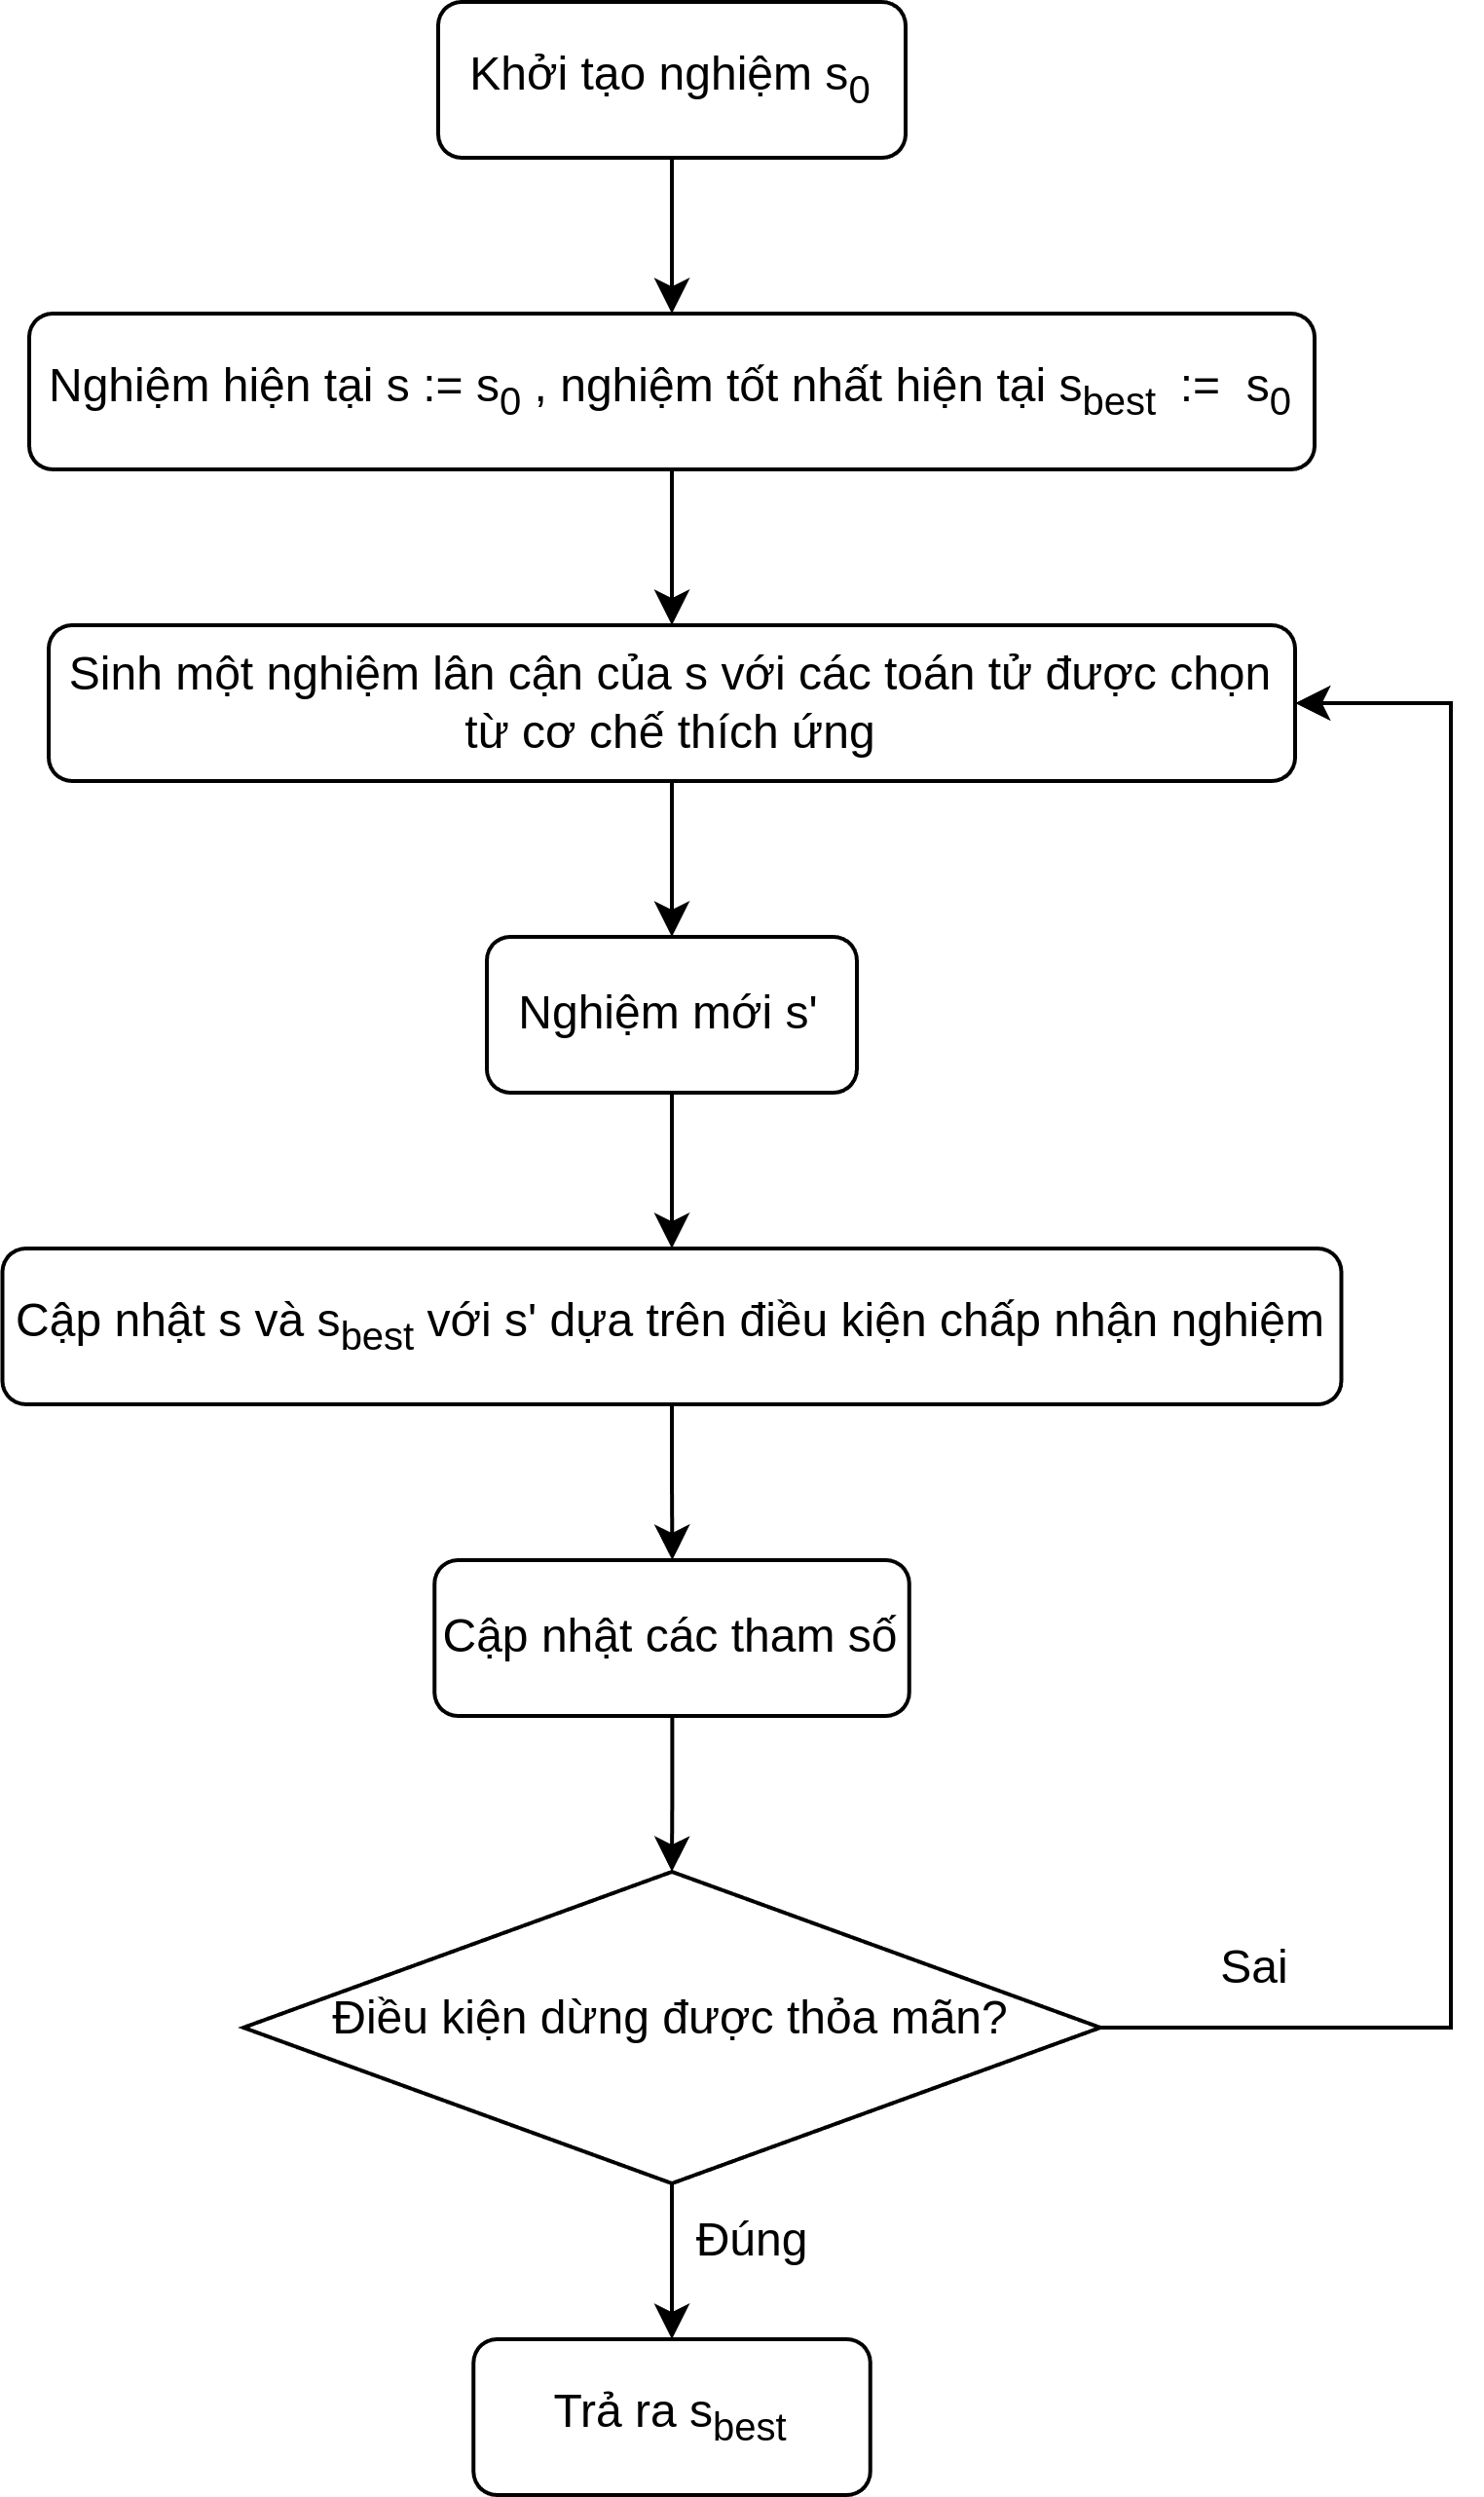
\includegraphics[width=0.6\textwidth]{figures/ALNS-flowchart.png} 
  % \includesvg[scale=1]{figures/core-object}
  \caption{Lược đồ chính của ALNS} 
  % \label{fig:fg_02}
\end{figure}

\subsection{Các lớp chính}
\label{sec:core-objects}
Trước hết, chúng ta xây dựng các lớp chính. Các lớp được xây dựng với kiểu dữ liệu của ngôn ngữ \code{C++}, ta hoàn toàn có thể triển khai tương tự với các ngôn ngữ lập trình khác. Các kiểu số nguyên được sử dụng là \code{uint16\_t} với giá trị lớn nhất là $65535$ (đủ lớn để lưu số lượng khách hàng thực tế cũng như nhu cầu hay tải trọng của khách hàng...) để tiết kiệm bộ nhớ. Các kiểu số thực được sử dụng là \code{float} thay vì \code{double}. Đôi khi, trong một số bộ thư viện (như \code{Google OR-Tools} chẳng hạn), thay vì sử dụng số thực để lưu khoảng cách hay thời gian di chuyển giữa các yêu cầu hoặc giá trị hàm mục tiêu, số nguyên được sử dụng để tiết kiệm bộ nhớ cũng như tính toán nhanh hơn. Nếu cần nhiều hơn độ chính xác, ta có thể nhân tất cả với một hệ số ($1000$ chẳng hạn để đạt độ chính xác $3$ chữ số sau dấu chấm động) và chia lại khi nhận kết quả cuối cùng. Các lớp được liệt kê dưới đây cùng với giải thích cụ thể của từng thuộc tính và phương thức.

\begin{figure}[H] % places figure environment here   
	\centering % Centers Graphic
	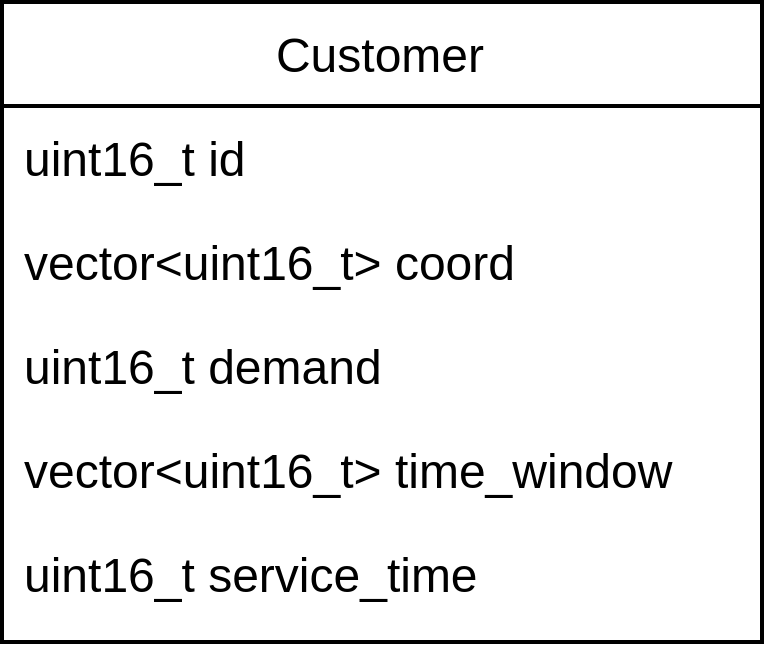
\includegraphics[width=0.35\textwidth]{figures/Customer.png}
	% \includesvg[scale=1]{figures/core-object}
	\caption{Lớp thuộc tính của khách hàng}
	\label{fig:fg_02}
\end{figure}

\code{Customer}: lớp lưu các thuộc tính của một yêu cầu. Đối với VRPTW, mỗi yêu cầu là một khách hàng (đơn).

\begin{itemize}
	\item[-] \code{id}: id của khách hàng.
	\item[-] \code{coord}: mảng lưu toạ độ của khách hàng (vĩ độ, kinh độ). Đôi khi chúng ta không cần quan tâm tới tọa độ của khách hàng mà quan tâm tới khoảng cách hoặc thời gian di chuyển giữa các khách hàng, nên thuộc tính này có thể không cần thiết đối với một số cấu hình trong thực tế.
	\item[-] \code{demand}: nhu cầu (về tải) của khách hàng.
	\item[-] \code{time\_window}: mảng lưu khung thời gian để phục vụ khách hàng. Mảng gồm 2 phần tử lần lượt là thời điểm sớm nhất và muộn nhất để phục vụ khách hàng.
	\item[-] \code{service\_time}: thời gian phục vụ khách hàng.
\end{itemize}


\code{CustomerRoute}: lớp lưu trạng thái về tuyến đường.
\begin{itemize}
	\item[-] \code{route\_idx}: id của tuyến chứa khách hàng.
	\item[-] \code{position}: vị trí của khách hàng trong tuyến.
\end{itemize}

\code{CustomerTime}: lớp lưu trạng thái về thời gian của yêu cầu.
\begin{itemize}
	\item[-] \code{arrival}: thời gian xe đến vị trí của khách hàng.
	\item[-] \code{complete}: thời gian xe hoàn thành phục vụ khách hàng.
\end{itemize}

\begin{figure}[H] % places figure environment here   
	\centering % Centers Graphic
	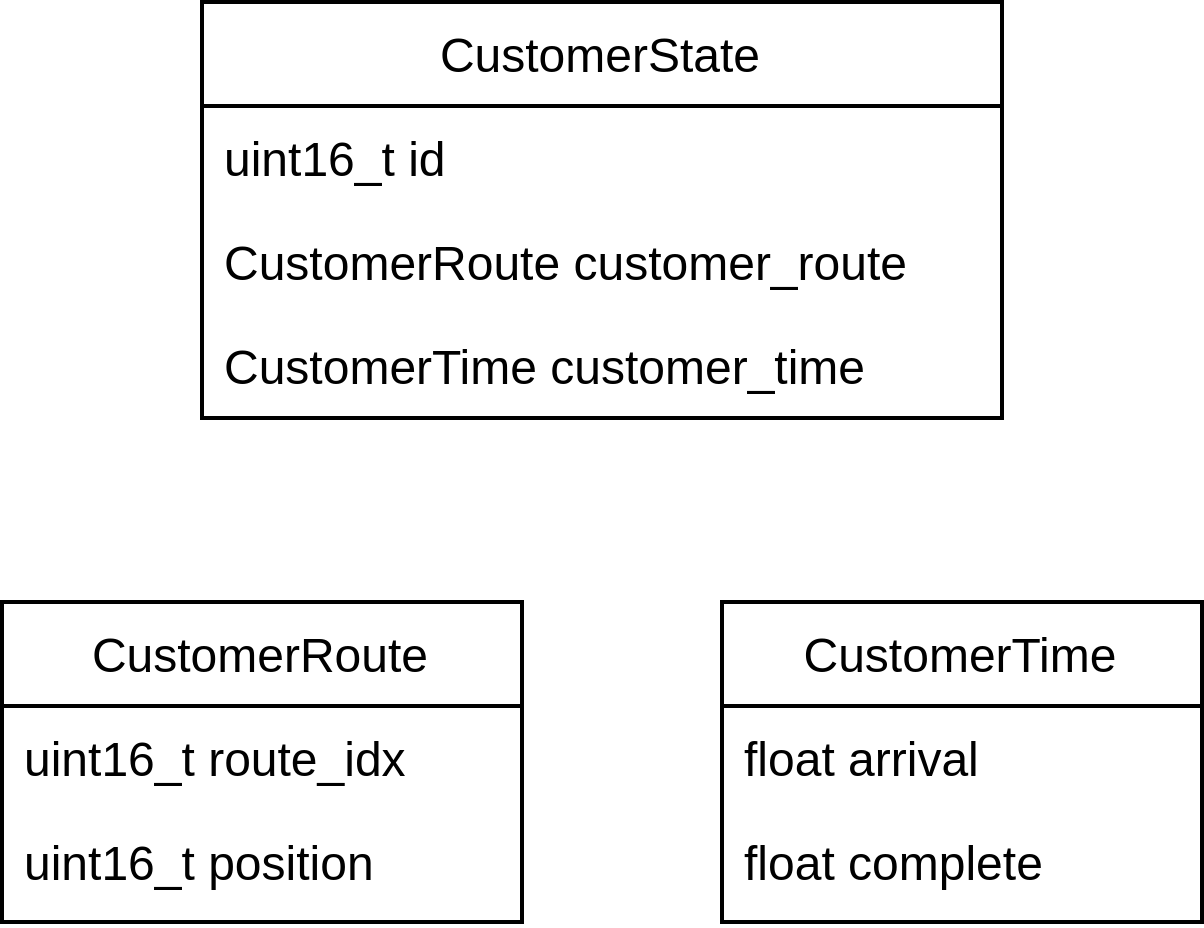
\includegraphics[width=0.6\textwidth]{figures/CustomerState.png}
	% \includesvg[scale=1]{figures/core-object}
	\caption{Lớp trạng thái của khách hàng}
	\label{fig:fg_03}
\end{figure}

\code{CustomerState}: lớp lưu trạng thái của khách hàng.
\begin{itemize}
	\item[-] \code{id}: id của khách hàng.
	\item[-] \code{customer\_route}: trạng thái về tuyến đường của khách hàng.
	\item[-] \code{customer\_time}: trạng thái về thời gian của khách hàng.
\end{itemize}

\begin{figure}[H] % places figure environment here   
	\centering % Centers Graphic
	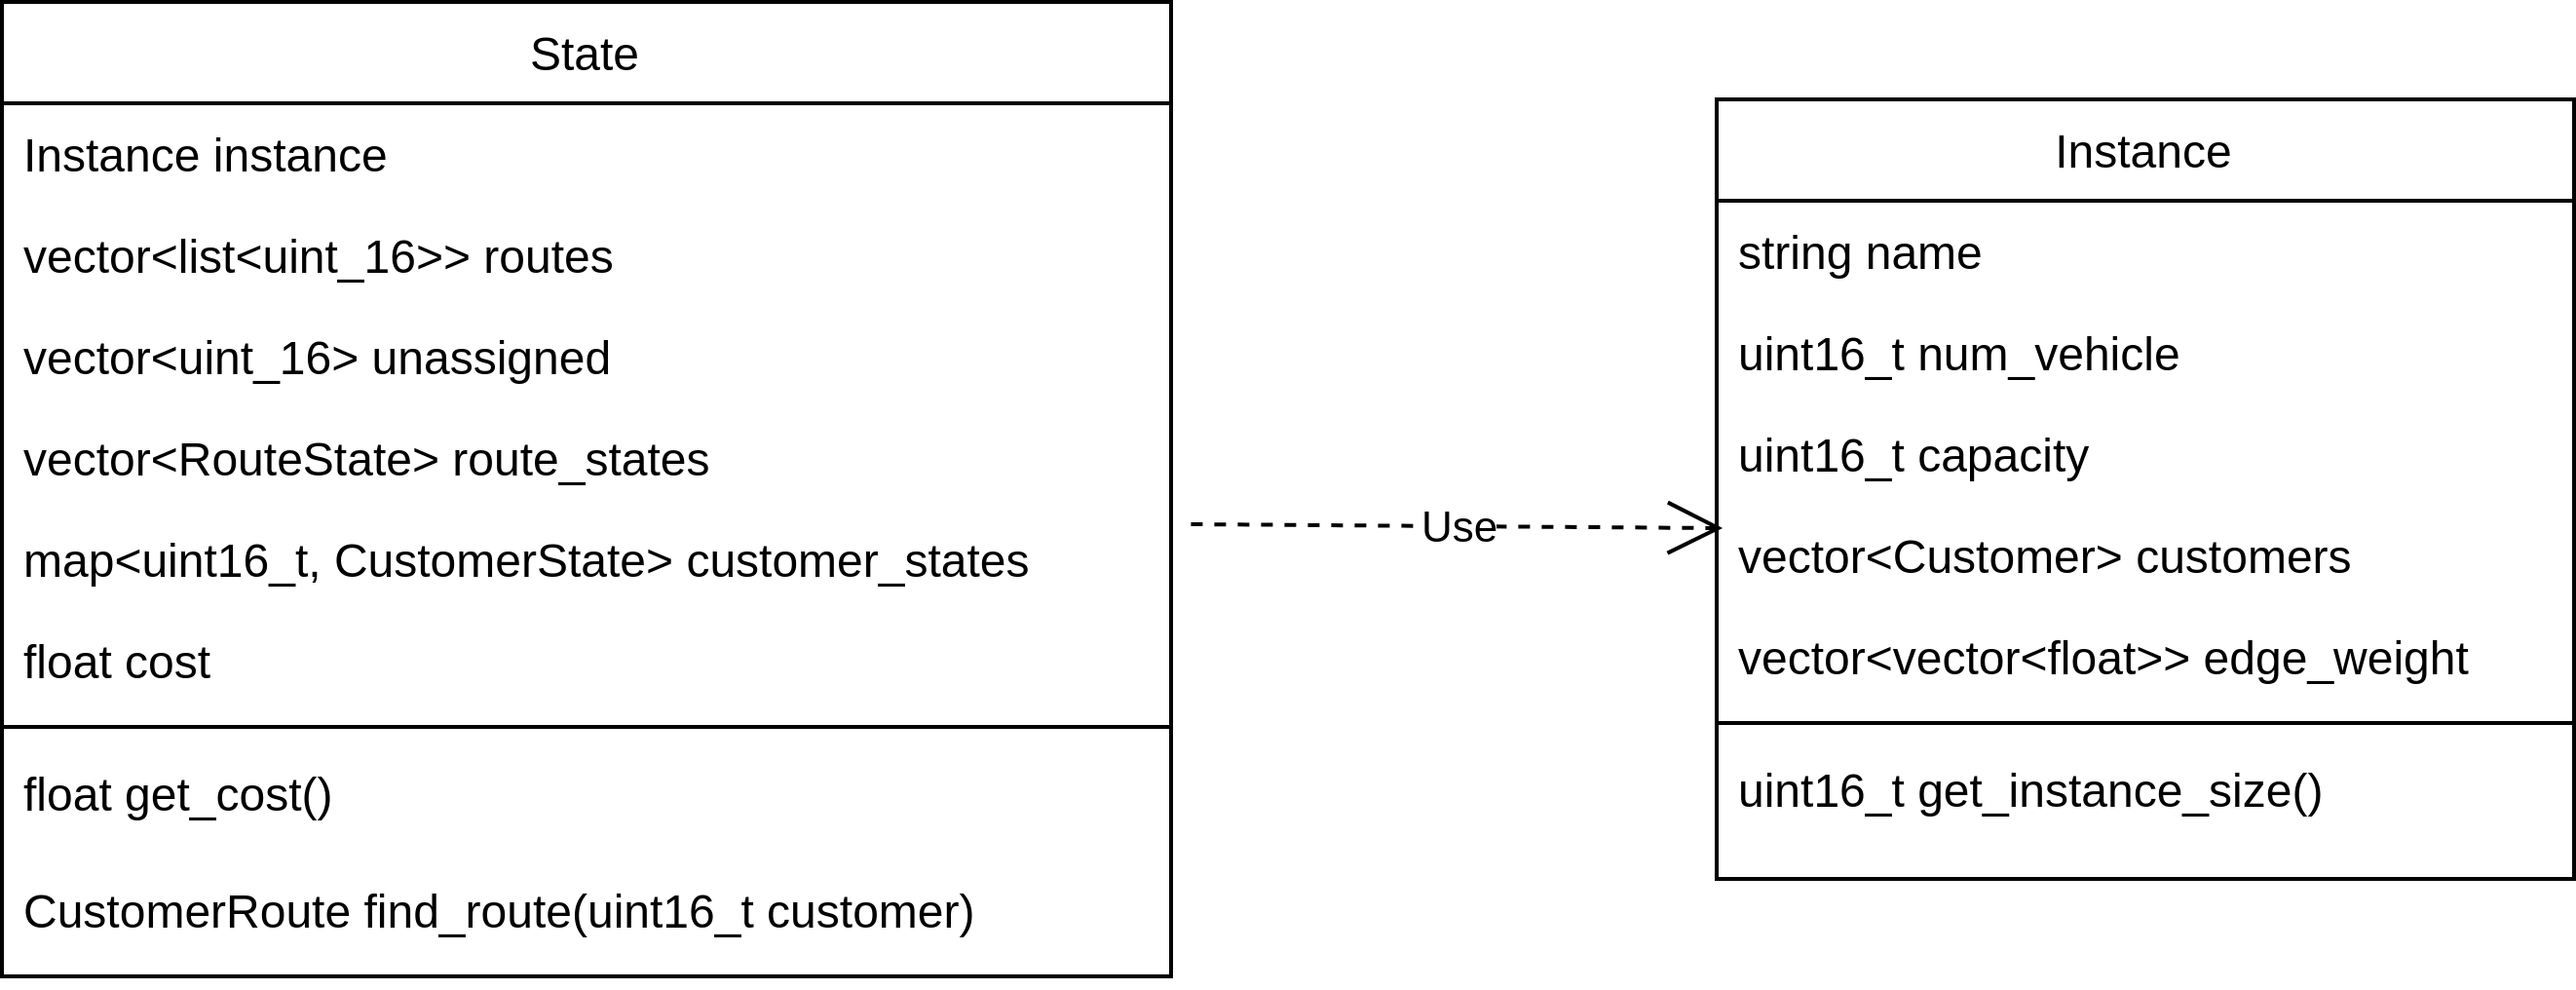
\includegraphics[width=1\textwidth]{figures/core-object.png}
	% \includesvg[scale=1]{figures/core-object}
	\caption{Lớp trạng thái của hệ}
	\label{fig:fg_04}
\end{figure}

\code{Instance}: lớp lưu cấu hình của bài toán.
\begin{itemize}
	\item[-] \code{name}: tên cấu hình (ví dụ \code{C101} trong tập Solomon (1987)).
	\item[-] \code{num\_vehicle}: số xe tối đa được sử dụng.
	\item[-] \code{capacity}: tải trọng của mỗi xe.
	\item[-] \code{customers}: mảng các yêu cầu.
	\item[-] \code{edge\_weight}: ma trận trọng số cạnh. Ma trận này có thể là ma trận khoảng cách hay thời gian di chuyển giữa các yêu cầu.
	\item[-] \code{get\_instance\_size()}: phương thức trả về kích thước của cấu hình (số khách hàng cộng với kho).
\end{itemize}

\code{State}: lớp lưu trạng thái của bài toán.
\begin{itemize}
	\item[-] \code{instance}: tham chiếu tới cấu hình bài toán.
	\item[-] \code{routes}: các tuyến đường. Các tuyến đường được tổ chức như một \code{vector} với mỗi thành phần là một \code{linked\_list}. Cấu trúc dữ liệu \code{linked\_list} được lựa chọn phù hợp với ALNS khi ta có thể  bỏ đi hoặc chèn thêm các yêu cầu vào giữa tuyến một cách nhanh chóng. Trong nhiều thuật toán khác, các yêu cầu được trao đổi giữa các tuyến thì \code{vector} là phù hợp hơn do ta có thể truy cập đến phần từ (yêu cầu) theo index rất nhanh mà không phải duyệt lần lượt từ đầu mảng giống như \code{linked\_list}. Việc sử dụng \code{linked\_list} cho ALNS là cực kì phù hợp, thao bỏ đi hay chèn thêm phần tử vào giữa tuyến nhanh hơn khoảng $250$ lần khi so sánh với việc sử dụng cấu trúc dữ liệu \code{vector}!
	\item[-] \code{unassigned}: danh sách các khách hàng chưa được phục vụ bởi bất kì xe nào.
	\item[-] \code{customer\_states}: trạng thái của các khách hàng.
	\item[-] \code{cost}: tổng chi phí của hệ (hay nghiệm) hiện tại.
	\item[-] \code{get\_cost()}: phương thức trả về cost hiên tại.
	\item[-] \code{find\_route(customer)}: phương thức trả về trạng thái của một khách hàng với đầu vào là id của khách hàng.
\end{itemize}
\section{Triển khai thuật toán}
Chương trình được chia làm ba giai đoạn \textit{Tiền xử lý}, \textit{Chương trình chính}, \textit{Đo đạc}.
\begin{itemize}
	\item \textit{Tiền xử lý}: trong giai đoạn này, các cấu hình trong các tập dữ liệu, được đọc vào và tính toán ma trận khoảng cách giữa các yêu cầu và lưu trữ vào các tệp. Các tệp có định dạng json và có schema như đối tượng \code{Instance} đã trình được trình bày trong mục \ref{sec:core-objects}. Các tệp này sẽ được đọc vào trong giai đoạn \textit{Chương trình chính} để giảm thiểu thời gian tính toán. Để đơn giản, phần tiền xử lý sử dụng ngôn ngữ lập trình \code{python}.
	\item \textit{Chương trình chính}: Đây là chương trình triển khai ALNS, được viết bằng ngôn ngữ \code{C++}. Các độ đo của chương trình được ghi ra các tệp logs để sử dụng cho giai đoạn \textit{đo đạc}.
	\item \textit{Đo đạc}: Trong giai đoạn này, các tệp logs được đọc vào và các độ đo được tính toán và phân tích.
\end{itemize}

Một trong những điểm mạnh của ALNS là triển khai được song song. Chúng ta có thể chạy nhiều luồng cùng một lúc để tăng tốc độ tính toán. Điều này đặc biệt hữu ích khi cấu hình cần giải có nhiều yêu cầu. Khi tìm kiếm nghiệm trong lân cận của nghiệm hiện tại, ta khởi tạo nhiều luồng cùng tìm kiếm. Điều này không những tăng tốc chương trình mà còn giúp cho thuật toán khó bị bẫy trong nghiệm tối ưu cục bộ hơn khi triển khai đơn luồng do sự đa dạng của việc tìm kiếm (bằng nhiều luồng). Ngoài ra có những cách triển khai đa luồng khác. Ví dụ, trong thuật toán "hủy" và "sửa", ta hoàn toàn có thể bỏ đi các yêu cầu hoặc thêm lại các yêu cầu một cách song song từ các tuyến đường khác nhau.

Trong thực tế, tác giả chọn cách triển khai đầu tiên vì đơn giản và dễ hiểu. Chúng ta chỉ cần khởi tạo các luồng một lần mà không cần phải cấp lại tài nguyên. Với cách làm thứ hai, ta liên tục phải tạo các luồng mới và cấp lại tài nguyên cho chúng, điều này có thể làm giảm hiệu năng của chương trình vì thực tế thì việc khởi tạo luồng là đắt đỏ. Tác giả cũng thử nghiệm cách làm thứ hai với thư viện \code{OpenMP} (là một thư viện hỗ trợ lập trình bất đồng bộ và song song nổi tiếng dành cho \code{C++}) tuy nhiên hiệu năng không đạt tốt như cách triển khai đa luồng đầu tiên.